% Template for PLoS
% Version 3.6 Aug 2022
%
% % % % % % % % % % % % % % % % % % % % % %
%
% -- IMPORTANT NOTE
%
% This template contains comments intended 
% to minimize problems and delays during our production 
% process. Please follow the template instructions
% whenever possible.
%
% % % % % % % % % % % % % % % % % % % % % % % 
%
% Once your paper is accepted for publication, 
% PLEASE REMOVE ALL TRACKED CHANGES in this file 
% and leave only the final text of your manuscript. 
% PLOS recommends the use of latexdiff to track changes during review, as this will help to maintain a clean tex file.
% Visit https://www.ctan.org/pkg/latexdiff?lang=en for info or contact us at latex@plos.org.
%
%
% There are no restrictions on package use within the LaTeX files except that no packages listed in the template may be deleted.
%
% Please do not include colors or graphics in the text.
%
% The manuscript LaTeX source should be contained within a single file (do not use \input, \externaldocument, or similar commands).
%
% % % % % % % % % % % % % % % % % % % % % % %
%
% -- FIGURES AND TABLES
%
% Please include tables/figure captions directly after the paragraph where they are first cited in the text.
%
% DO NOT INCLUDE GRAPHICS IN YOUR MANUSCRIPT
% - Figures should be uploaded separately from your manuscript file. 
% - Figures generated using LaTeX should be extracted and removed from the PDF before submission. 
% - Figures containing multiple panels/subfigures must be combined into one image file before submission.
% For figure citations, please use "Fig" instead of "Figure".
% See http://journals.plos.org/plosone/s/figures for PLOS figure guidelines.
%
% Tables should be cell-based and may not contain:
% - spacing/line breaks within cells to alter layout or alignment
% - do not nest tabular environments (no tabular environments within tabular environments)
% - no graphics or colored text (cell background color/shading OK)
% See http://journals.plos.org/plosone/s/tables for table guidelines.
%
% For tables that exceed the width of the text column, use the adjustwidth environment as illustrated in the example table in text below.
%
% % % % % % % % % % % % % % % % % % % % % % % %
%
% -- EQUATIONS, MATH SYMBOLS, SUBSCRIPTS, AND SUPERSCRIPTS
%
% IMPORTANT
% Below are a few tips to help format your equations and other special characters according to our specifications. For more tips to help reduce the possibility of formatting errors during conversion, please see our LaTeX guidelines at http://journals.plos.org/plosone/s/latex
%
% For inline equations, please be sure to include all portions of an equation in the math environment.  For example, x$^2$ is incorrect; this should be formatted as $x^2$ (or $\mathrm{x}^2$ if the romanized font is desired).
%
% Do not include text that is not math in the math environment. For example, CO2 should be written as CO\textsubscript{2} instead of CO$_2$.
%
% Please add line breaks to long display equations when possible in order to fit size of the column. 
%
% For inline equations, please do not include punctuation (commas, etc) within the math environment unless this is part of the equation.
%
% When adding superscript or subscripts outside of brackets/braces, please group using {}.  For example, change "[U(D,E,\gamma)]^2" to "{[U(D,E,\gamma)]}^2". 
%
% Do not use \cal for caligraphic font.  Instead, use \mathcal{}
%
% % % % % % % % % % % % % % % % % % % % % % % % 
%
% Please contact latex@plos.org with any questions.
%
% % % % % % % % % % % % % % % % % % % % % % % %

\documentclass[10pt,letterpaper]{article}
%\documentclass[10pt]{article}
%\usepackage[top=0.85in,left=2.75in,footskip=0.75in]{geometry}

\usepackage[paper=a4paper,
  inner=2.5cm,
  outer=3.8cm,
  bindingoffset=.5cm,
  top=1.5cm,
  bottom=1.5cm]{geometry}


% amsmath and amssymb packages, useful for mathematical formulas and symbols
\usepackage{amsmath,amssymb}
\usepackage{physics}
\newcommand{\pdvn}[3]{\frac{\partial^{#1} {#2}}{\partial {#3}^{#1}}}
\newcommand{\Underbrace}[2]{{\underbrace{#2}_{#1}}}

% Use adjustwidth environment to exceed column width (see example table in text)
\usepackage{changepage}

% textcomp package and marvosym package for additional characters
\usepackage{textcomp,marvosym}

% cite package, to clean up citations in the main text. Do not remove.
% \usepackage{cite}

% Use nameref to cite supporting information files (see Supporting Information section for more info)
\usepackage{nameref,hyperref}

% line numbers
\usepackage[right]{lineno}

% ligatures disabled
\usepackage[nopatch=eqnum]{microtype}
\DisableLigatures[f]{encoding = *, family = * }

% color can be used to apply background shading to table cells only
\usepackage[table]{xcolor}

% array package and thick rules for tables
\usepackage{array}

% create "+" rule type for thick vertical lines
\newcolumntype{+}{!{\vrule width 2pt}}

% create \thickcline for thick horizontal lines of variable length
\newlength\savedwidth
\newcommand\thickcline[1]{%
  \noalign{\global\savedwidth\arrayrulewidth\global\arrayrulewidth 2pt}%
  \cline{#1}%
  \noalign{\vskip\arrayrulewidth}%
  \noalign{\global\arrayrulewidth\savedwidth}%
}


% \thickhline command for thick horizontal lines that span the table
\newcommand\thickhline{\noalign{\global\savedwidth\arrayrulewidth\global\arrayrulewidth 2pt}%
\hline
\noalign{\global\arrayrulewidth\savedwidth}}


% Remove comment for double spacing
\usepackage{setspace} 
\doublespacing

% Text layout
\raggedright
\setlength{\parindent}{0.5cm}
\textwidth 5.25in
\textheight 8.75in

% Bold the 'Figure #' in the caption and separate it from the title/caption with a period
% Captions will be left justified
\usepackage[aboveskip=1pt,labelfont=bf,labelsep=period,justification=raggedright,singlelinecheck=off]{caption}
\renewcommand{\figurename}{Fig}
  
% Use the PLoS provided BiBTeX style
% \bibliographystyle{plos2015}
% Remove brackets from numbering in List of References

\makeatletter
\renewcommand{\@biblabel}[1]{\quad#1.}
\makeatother




% Header and Footer with logo

\usepackage{lastpage,fancyhdr,graphicx}
\usepackage{epstopdf}
\usepackage[bibstyle=numeric,style=authoryear-icomp,maxbibnames=10,maxcitenames=2,uniquelist=false, backend=bibtex,url=false, sorting=none]{biblatex}
\usepackage{float}



\addbibresource{manual.bib}
\AtEveryBibitem{\clearfield{note}}



%\addbibresource{Mendeley.bib}
%\addbibresource{manual.bib}
%\bibliography{references}
%\pagestyle{myheadings}
\pagestyle{fancy}
\fancyhf{}
%\setlength{\headheight}{27.023pt}
%\lhead{\includegraphics[width=2.0in]{PLOS-submission.eps}}
\rfoot{\thepage/\pageref{LastPage}}
\renewcommand{\headrulewidth}{0pt}
\renewcommand{\footrule}{\hrule height 2pt \vspace{2mm}}
\fancyheadoffset[L]{2.25in}
\fancyfootoffset[L]{2.25in}
\lfoot{\today}

%% Include all macros below

\newcommand{\lorem}{{\bf LOREM}}
\newcommand{\ipsum}{{\bf IPSUM}}

%% END MACROS SECTION

\setlength{\parskip}{\baselineskip}%
\setlength{\parindent}{0pt}%
\begin{document}
\vspace*{0.2in}

% Title must be 250 characters or less.
\begin{flushleft}
{\Large
\textbf\newline{Effects of multistability, absorbing boundaries and growth on Turing pattern formation} % Please use "sentence case" for title and headings (capitalize only the first word in a title (or heading), the first word in a subtitle (or subheading), and any proper nouns).
}
\newline
% Insert author names, affiliations and corresponding author email (do not include titles, positions, or degrees).
\\
Martina Oliver Huidobro \textsuperscript{1},
Robert G. Endres \textsuperscript{1}


\bigskip
\textbf{1} Department of Life Sciences and Centre for Integrative Systems Biology and Bioinformatics, Imperial College, London, United Kingdom
\\
\bigskip

% Insert additional author notes using the symbols described below. Insert symbol callouts after author names as necessary.
% 
% Remove or comment out the author notes below if they aren't used.
%
% Primary Equal Contribution Note
%\Yinyang These authors contributed equally to this work.

% Additional Equal Contribution Note
% Also use this double-dagger symbol for special authorship notes, such as senior authorship.
%\ddag These authors also contributed equally to this work.

% Current address notes
%\textcurrency Current Address: Life Sciences Department, Imperial College London, London, United Kingdom% change symbol to "\textcurrency a" if more than one current address note
% \textcurrency b Insert second current address 
% \textcurrency c Insert third current address

% Deceased author note
%\dag Deceased

% Group/Consortium Author Note
%\textpilcrow Membership list can be found in the Acknowledgments section.

% Use the asterisk to denote corresponding authorship and provide email address in note below.

* r.endres@imperial.ac.uk

\end{flushleft}
% Please keep the abstract below 300 words

%\section*{Supporting information}
%
%% Include only the SI item label in the paragraph heading. Use the \nameref{label} command to cite SI items in the text.
%\paragraph*{S1 Fig.}
%\label{S1_Fig}
%{\bf Bold the title sentence.} Add descriptive text after the title of the item (optional).
%
%\paragraph*{S2 Fig.}
%\label{S2_Fig}
%{\bf Lorem ipsum.} Maecenas convallis mauris sit amet sem ultrices gravida. Etiam eget sapien nibh. Sed ac ipsum eget enim egestas ullamcorper nec euismod ligula. Curabitur fringilla pulvinar lectus consectetur pellentesque.
%
%\paragraph*{S1 File.}
%\label{S1_File}
%{\bf Lorem ipsum.}  Maecenas convallis mauris sit amet sem ultrices gravida. Etiam eget sapien nibh. Sed ac ipsum eget enim egestas ullamcorper nec euismod ligula. Curabitur fringilla pulvinar lectus consectetur pellentesque.
%
%\paragraph*{S1 Video.}
%\label{S1_Video}
%{\bf Lorem ipsum.}  Maecenas convallis mauris sit amet sem ultrices gravida. Etiam eget sapien nibh. Sed ac ipsum eget enim egestas ullamcorper nec euismod ligula. Curabitur fringilla pulvinar lectus consectetur pellentesque.
%
%\paragraph*{S1 Appendix.}
%\label{S1_Appendix}
%{\bf Lorem ipsum.} Maecenas convallis mauris sit amet sem ultrices gravida. Etiam eget sapien nibh. Sed ac ipsum eget enim egestas ullamcorper nec euismod ligula. Curabitur fringilla pulvinar lectus consectetur pellentesque.
%
%\paragraph*{S1 Table.}
%\label{S1_Table}
%{\bf Lorem ipsum.} Maecenas convallis mauris sit amet sem ultrices gravida. Etiam eget sapien nibh. Sed ac ipsum eget enim egestas ullamcorper nec euismod ligula. Curabitur fringilla pulvinar lectus consectetur pellentesque.
%
%\section*{Acknowledgments}
%Cras egestas velit mauris, eu mollis turpis pellentesque sit amet. Interdum et malesuada fames ac ante ipsum primis in faucibus. Nam id pretium nisi. Sed ac quam id nisi malesuada congue. Sed interdum aliquet augue, at pellentesque quam rhoncus vitae.
%
%\nolinenumbers
%
%% Either type in your references using
%% \begin{thebibliography}{}
%% \bibitem{}
%% Text
%% \end{thebibliography}
%%
%% or
%%
%% Compile your BiBTeX database using our plos2015.bst
%% style file and paste the contents of your .bbl file
%% here. See http://journals.plos.org/plosone/s/latex for
%% step-by-step instructions.
%%
%\begin{thebibliography}{10}
%
%\bibitem{bib1}
%Conant GC, Wolfe KH.
%\newblock {{T}urning a hobby into a job: how duplicated genes find new
%  functions}.
%\newblock Nat Rev Genet. 2008 Dec;9(12):938--950.
%
%\bibitem{bib2}
%Ohno S.
%\newblock Evolution by gene duplication.
%\newblock London: George Alien \& Unwin Ltd. Berlin, Heidelberg and New York:
%  Springer-Verlag.; 1970.
%
%\bibitem{bib3}
%Magwire MM, Bayer F, Webster CL, Cao C, Jiggins FM.
%\newblock {{S}uccessive increases in the resistance of {D}rosophila to viral
%  infection through a transposon insertion followed by a {D}uplication}.
%\newblock PLoS Genet. 2011 Oct;7(10):e1002337.

%\end{thebibliography}

\printbibliography[heading=bibintoc]
\section{Supplementary Material}
\newcommand{\beginsupplement}{%
    \setcounter{table}{0}
    \renewcommand{\thetable}{S\arabic{table}}%
    \setcounter{figure}{0}
    \renewcommand{\thefigure}{S\arabic{figure}}%
}
\beginsupplement

\begin{figure}[!ht]
    \center
    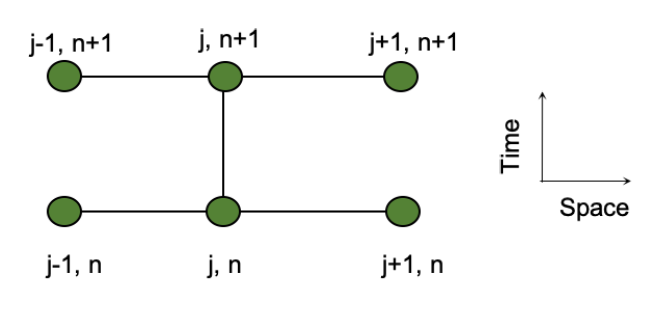
\includegraphics[width=0.3\textwidth]{figures/stencils}

    \caption{\textbf{Crank-Nicolson (CN) algorithm for numerical solution}. A stencil is a geometric representation with nodes and edges that represents the points of interest for the numerical approximation. The points of interest, which are the ones present in the equations, are shown in green. Labels $j$ and $n$ are the current space and time points. The CN stencil has one spatial dimension and one temporal dimension, with axes labels time and space ($x$). }   \label{sup_fig1}
\end{figure}


\begin{figure}[!h]
    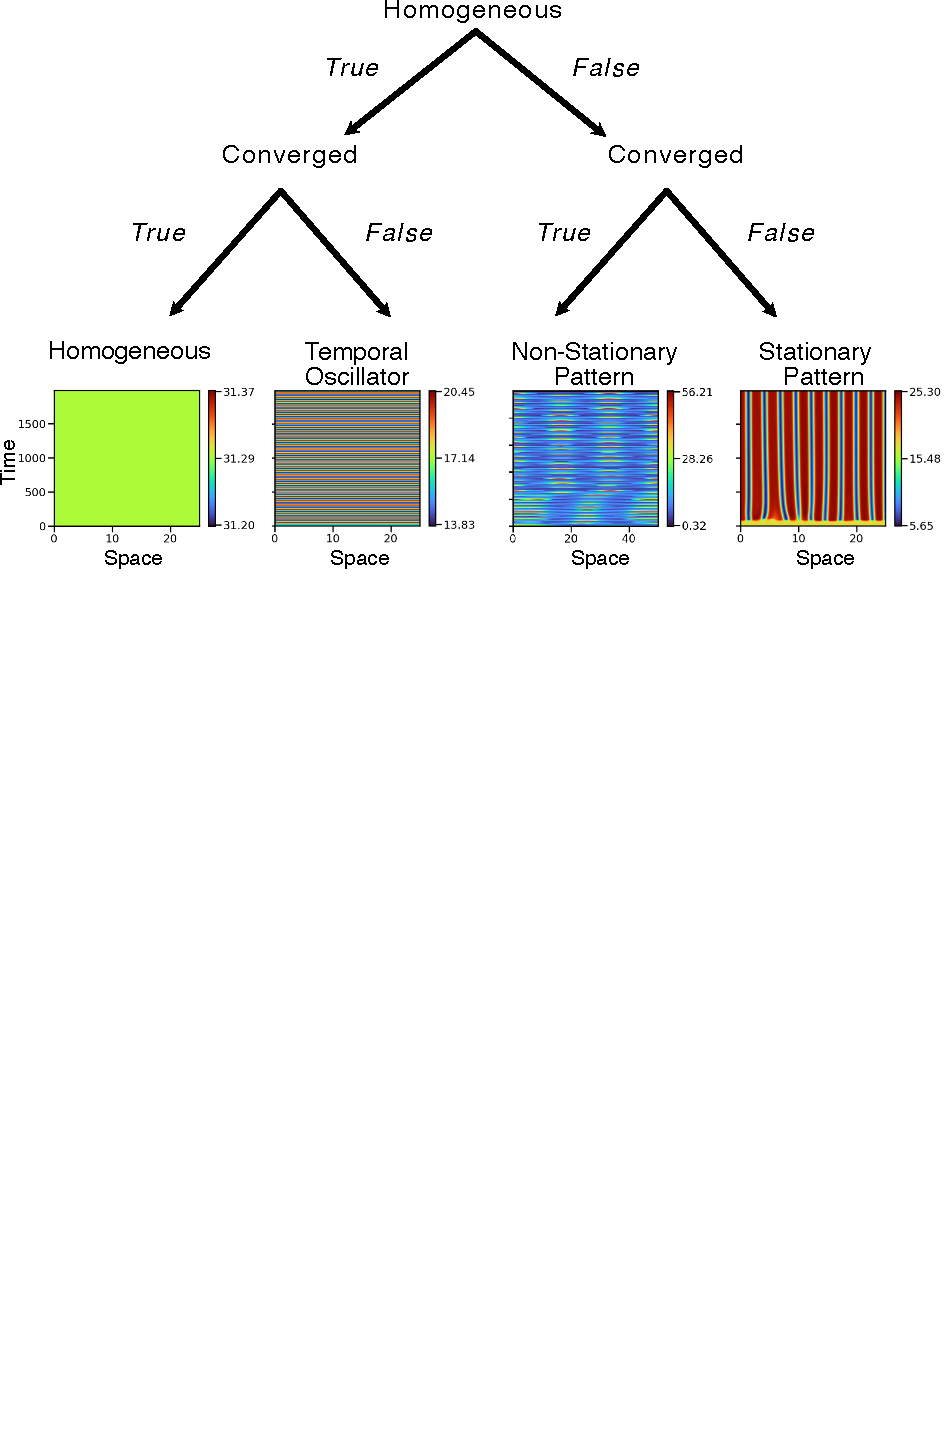
\includegraphics[width=1\textwidth]{figures/no_growth_classification}

    \caption{\textbf{Decision tree for pattern classification in non-growing domains with reflective boundaries}. A decision tree is based on two layers: spatial homogeneity and convergence. The numerical solutions for the four different pattern outcomes including  homogeneous, temporal oscillator, non-stationary, and stationary pattern as shown below.}
    \label{sup_fig2}
\end{figure}


\begin{figure}[!h]
    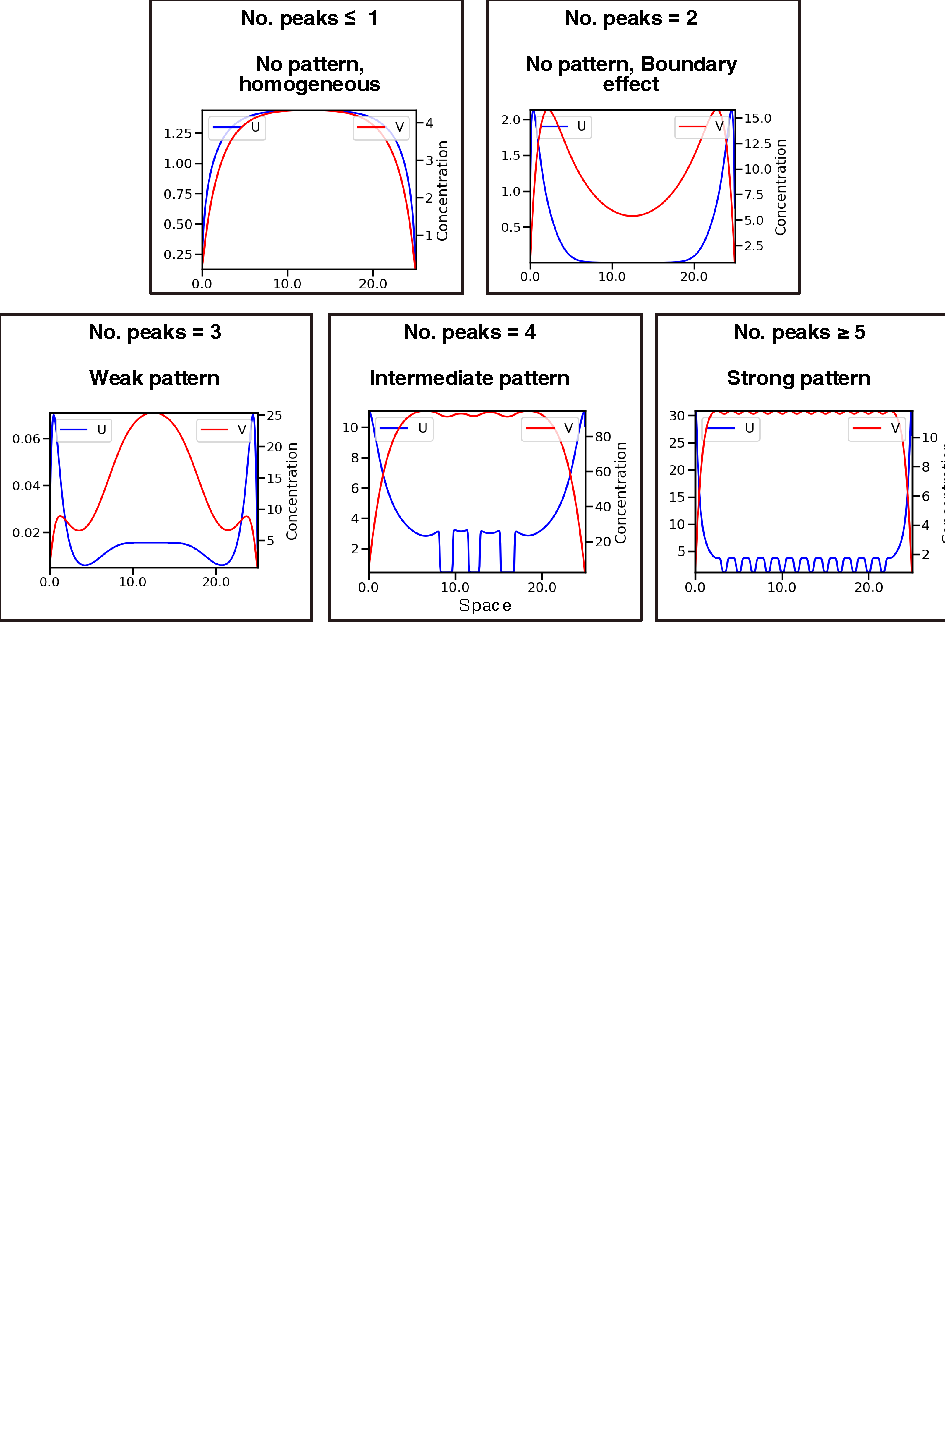
\includegraphics[width=1\textwidth]{figures/growth_classification}

    \caption{\textbf{Decision tree for pattern classification in non-growing domains with reflective boundaries}. A decision tree is based on two layers: spatial homogeneity and convergence. The numerical solutions for the four different pattern outcomes including  homogeneous, temporal oscillator, non-stationary, and stationary pattern as shown below.}
    \label{sup_fig3}
\end{figure}


\begin{figure}[!h]
    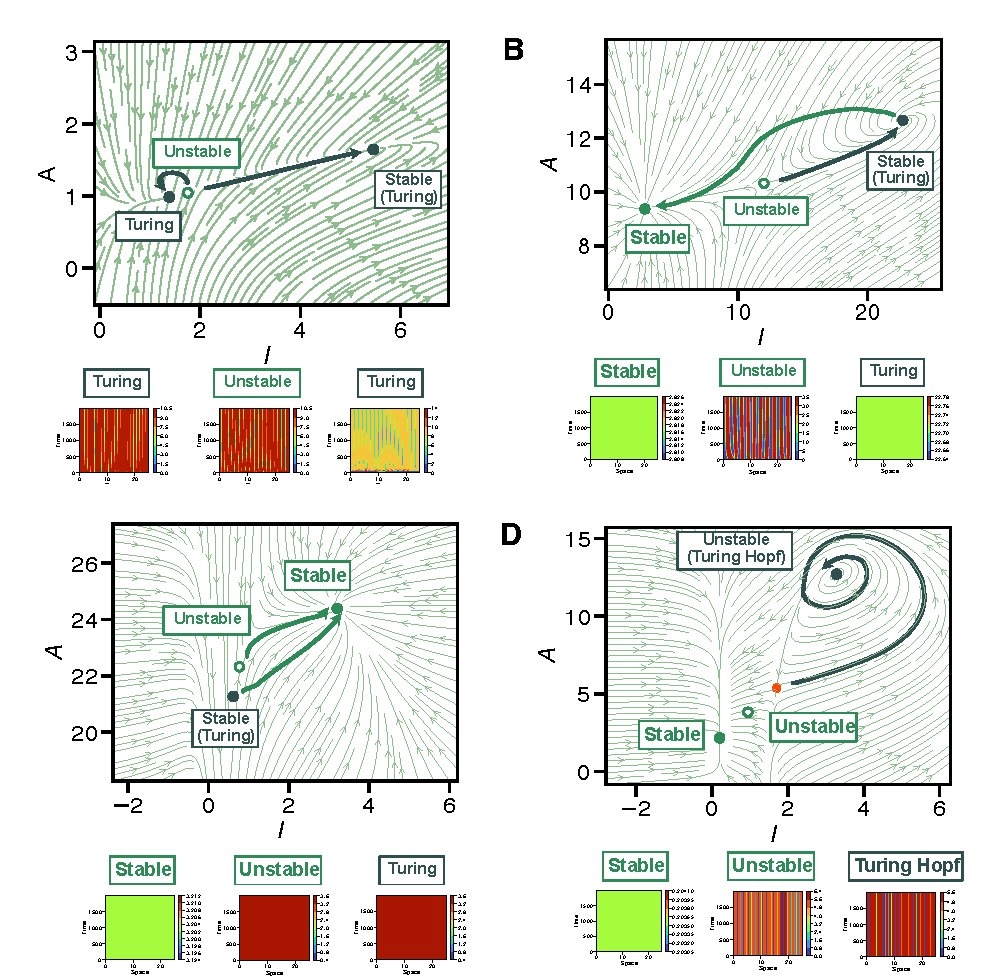
\includegraphics[width=1\textwidth]{figures/multistability_leftovers}

    \caption{\textbf{Other types of multistability dynamics.} \textbf{(A)} Unstable state converges into Turing. \textbf{(B)} Unstable state produces pattern, while Turing state loses pattern. \textbf{(C)} Multistability disrupts all patterns. \textbf{(D)} Turing I-Hopf state attracts unstable state and generates pattern.}

    \label{sup_fig4}
\end{figure}




\begin{figure}[!h]
    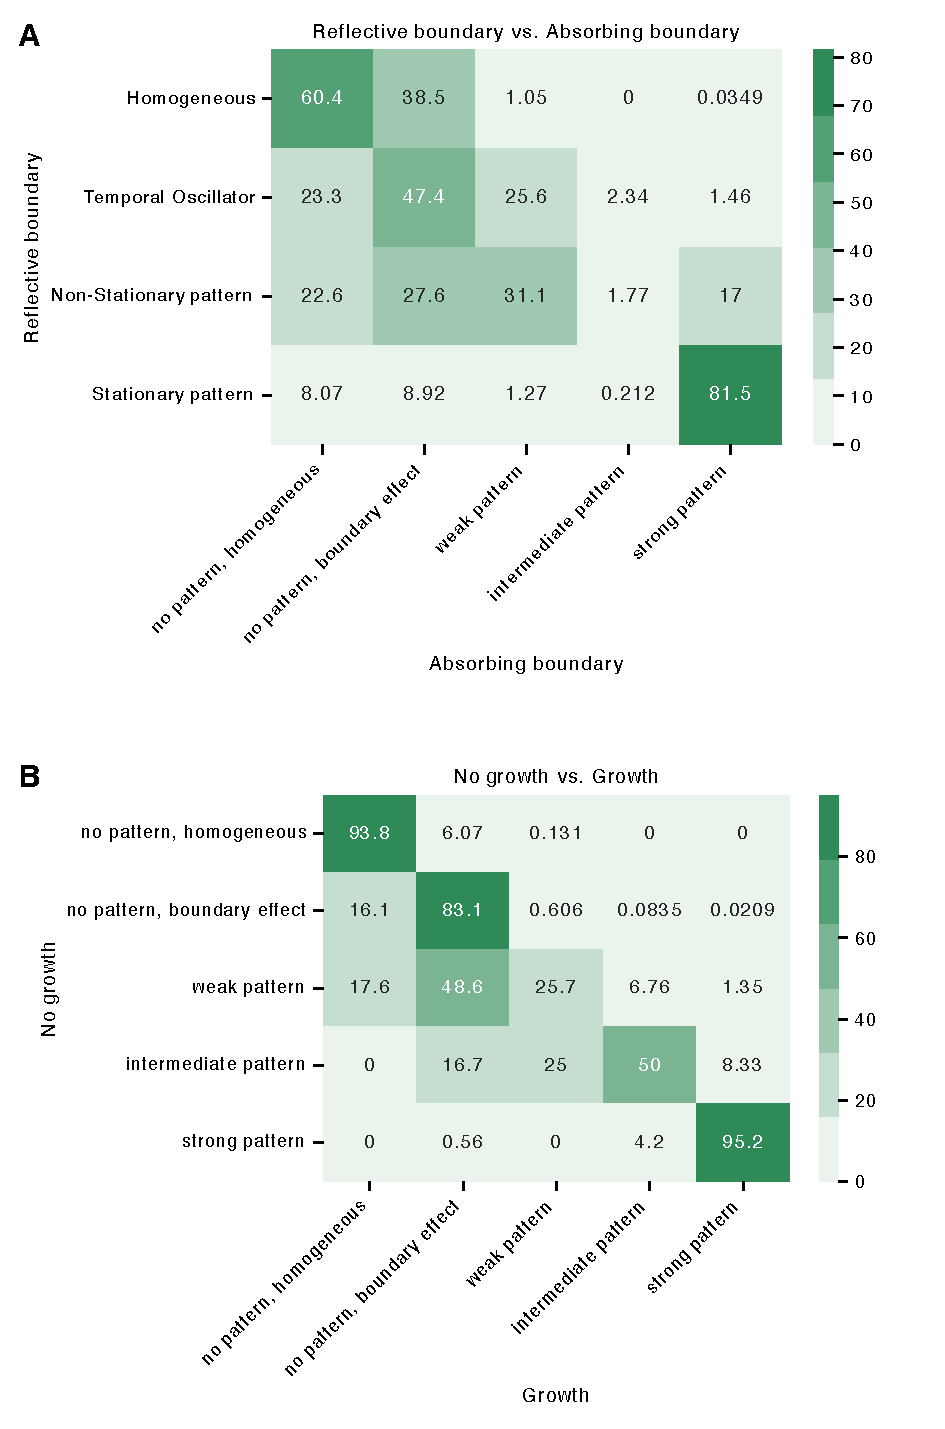
\includegraphics[width=1\textwidth]{figures/sup_confusion_matrix}

    \caption{\textbf{}}

    \label{sup_fig5}
\end{figure}


\end{document}

